% Created by tikzDevice version 0.12.6 on 2025-04-07 11:35:10
% !TEX encoding = UTF-8 Unicode
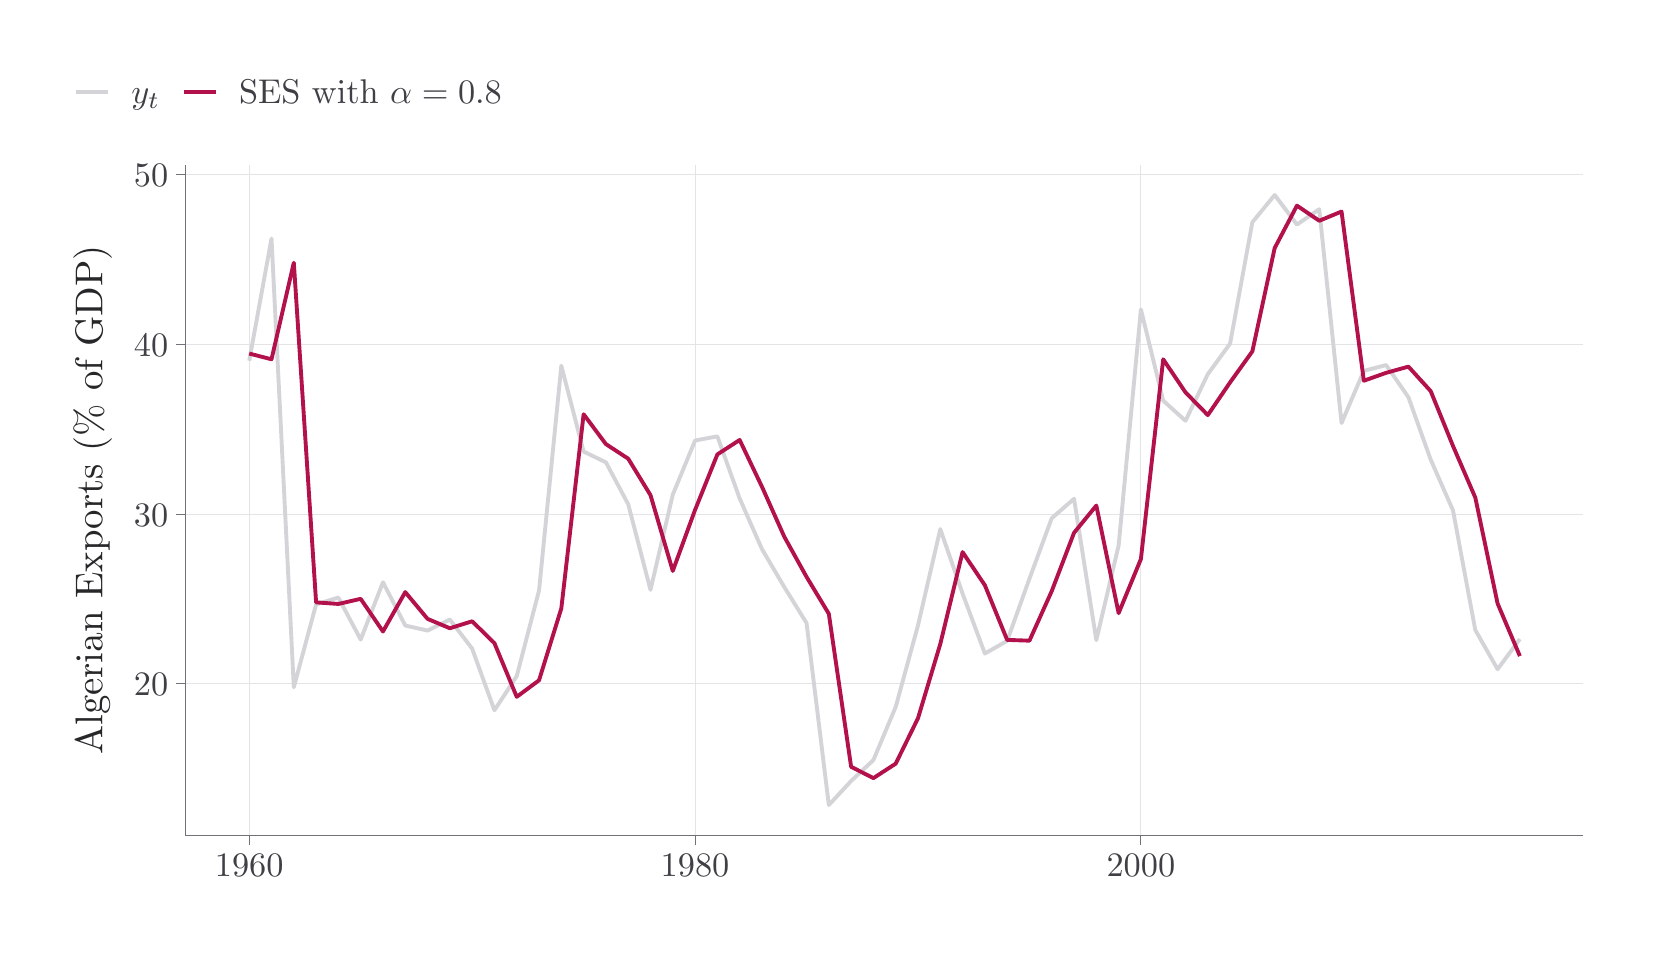
\begin{tikzpicture}[x=1pt,y=1pt]
\definecolor{fillColor}{RGB}{255,255,255}
\path[use as bounding box,fill=fillColor] (0,0) rectangle (578.16,325.21);
\begin{scope}
\path[clip] (  0.00,  0.00) rectangle (578.16,325.21);
\definecolor{drawColor}{RGB}{255,255,255}

\path[draw=drawColor,line width= 0.7pt,line join=round,line cap=round,fill=fillColor] (  0.00,  0.00) rectangle (578.16,325.21);
\end{scope}
\begin{scope}
\path[clip] ( 57.10, 33.29) rectangle (562.16,275.76);
\definecolor{drawColor}{RGB}{255,255,255}
\definecolor{fillColor}{RGB}{255,255,255}

\path[draw=drawColor,line width= 0.7pt,line join=round,line cap=round,fill=fillColor] ( 57.10, 33.29) rectangle (562.16,275.76);
\definecolor{drawColor}{RGB}{228,228,231}

\path[draw=drawColor,line width= 0.4pt,line join=round] ( 57.10, 88.11) --
	(562.16, 88.11);

\path[draw=drawColor,line width= 0.4pt,line join=round] ( 57.10,149.42) --
	(562.16,149.42);

\path[draw=drawColor,line width= 0.4pt,line join=round] ( 57.10,210.72) --
	(562.16,210.72);

\path[draw=drawColor,line width= 0.4pt,line join=round] ( 57.10,272.03) --
	(562.16,272.03);

\path[draw=drawColor,line width= 0.4pt,line join=round] ( 80.06, 33.29) --
	( 80.06,275.76);

\path[draw=drawColor,line width= 0.4pt,line join=round] (241.16, 33.29) --
	(241.16,275.76);

\path[draw=drawColor,line width= 0.4pt,line join=round] (402.26, 33.29) --
	(402.26,275.76);
\definecolor{drawColor}{RGB}{212,212,216}

\path[draw=drawColor,line width= 1.4pt,line join=round] ( 80.06,204.86) --
	( 88.11,249.01) --
	( 96.17, 86.85) --
	(104.22,116.83) --
	(112.28,119.28) --
	(120.33,104.08) --
	(128.39,124.81) --
	(136.44,109.17) --
	(144.50,107.34) --
	(152.55,111.34) --
	(160.61,100.82) --
	(168.66, 78.56) --
	(176.72, 90.87) --
	(184.78,121.85) --
	(192.83,203.06) --
	(200.89,172.03) --
	(208.94,168.14) --
	(217.00,153.01) --
	(225.05,122.05) --
	(233.11,156.46) --
	(241.16,176.02) --
	(249.22,177.54) --
	(257.27,155.09) --
	(265.33,136.80) --
	(273.38,123.12) --
	(281.44,110.08) --
	(289.49, 44.31) --
	(297.55, 53.00) --
	(305.60, 60.57) --
	(313.66, 79.77) --
	(321.71,109.22) --
	(329.77,144.01) --
	(337.82,120.72) --
	(345.88, 99.05) --
	(353.93,103.63) --
	(361.99,126.09) --
	(370.04,147.95) --
	(378.10,154.97) --
	(386.15,103.92) --
	(394.21,138.08) --
	(402.26,223.41) --
	(410.32,190.43) --
	(418.38,183.16) --
	(426.43,199.99) --
	(434.49,211.05) --
	(442.54,254.90) --
	(450.60,264.74) --
	(458.65,254.06) --
	(466.71,259.61) --
	(474.76,182.35) --
	(482.82,201.19) --
	(490.87,203.29) --
	(498.93,191.66) --
	(506.98,169.10) --
	(515.04,150.76) --
	(523.09,107.56) --
	(531.15, 93.38) --
	(539.20,104.29);
\definecolor{drawColor}{RGB}{179,17,75}

\path[draw=drawColor,line width= 1.4pt,line join=round] ( 80.06,207.45) --
	( 88.11,205.38) --
	( 96.17,240.28) --
	(104.22,117.54) --
	(112.28,116.97) --
	(120.33,118.82) --
	(128.39,107.02) --
	(136.44,121.25) --
	(144.50,111.58) --
	(152.55,108.19) --
	(160.61,110.71) --
	(168.66,102.80) --
	(176.72, 83.41) --
	(184.78, 89.38) --
	(192.83,115.36) --
	(200.89,185.52) --
	(208.94,174.73) --
	(217.00,169.46) --
	(225.05,156.30) --
	(233.11,128.90) --
	(241.16,150.95) --
	(249.22,171.00) --
	(257.27,176.23) --
	(265.33,159.32) --
	(273.38,141.30) --
	(281.44,126.76) --
	(289.49,113.42) --
	(297.55, 58.13) --
	(305.60, 54.03) --
	(313.66, 59.26) --
	(321.71, 75.67) --
	(329.77,102.51) --
	(337.82,135.71) --
	(345.88,123.72) --
	(353.93,103.98) --
	(361.99,103.70) --
	(370.04,121.61) --
	(378.10,142.68) --
	(386.15,152.52) --
	(394.21,113.64) --
	(402.26,133.19) --
	(410.32,205.37) --
	(418.38,193.42) --
	(426.43,185.21) --
	(434.49,197.03) --
	(442.54,208.25) --
	(450.60,245.57) --
	(458.65,260.90) --
	(466.71,255.43) --
	(474.76,258.77) --
	(482.82,197.63) --
	(490.87,200.48) --
	(498.93,202.73) --
	(506.98,193.87) --
	(515.04,174.05) --
	(523.09,155.42) --
	(531.15,117.13) --
	(539.20, 98.13);
\end{scope}
\begin{scope}
\path[clip] (  0.00,  0.00) rectangle (578.16,325.21);
\definecolor{drawColor}{RGB}{113,113,122}

\path[draw=drawColor,line width= 0.3pt,line join=round] ( 57.10, 33.29) --
	( 57.10,275.76);
\end{scope}
\begin{scope}
\path[clip] (  0.00,  0.00) rectangle (578.16,325.21);
\definecolor{drawColor}{RGB}{63,63,70}

\node[text=drawColor,anchor=base east,inner sep=0pt, outer sep=0pt, scale=  1.24] at ( 50.80, 83.83) {20};

\node[text=drawColor,anchor=base east,inner sep=0pt, outer sep=0pt, scale=  1.24] at ( 50.80,145.13) {30};

\node[text=drawColor,anchor=base east,inner sep=0pt, outer sep=0pt, scale=  1.24] at ( 50.80,206.44) {40};

\node[text=drawColor,anchor=base east,inner sep=0pt, outer sep=0pt, scale=  1.24] at ( 50.80,267.75) {50};
\end{scope}
\begin{scope}
\path[clip] (  0.00,  0.00) rectangle (578.16,325.21);
\definecolor{drawColor}{RGB}{113,113,122}

\path[draw=drawColor,line width= 0.3pt,line join=round] ( 53.60, 88.11) --
	( 57.10, 88.11);

\path[draw=drawColor,line width= 0.3pt,line join=round] ( 53.60,149.42) --
	( 57.10,149.42);

\path[draw=drawColor,line width= 0.3pt,line join=round] ( 53.60,210.72) --
	( 57.10,210.72);

\path[draw=drawColor,line width= 0.3pt,line join=round] ( 53.60,272.03) --
	( 57.10,272.03);
\end{scope}
\begin{scope}
\path[clip] (  0.00,  0.00) rectangle (578.16,325.21);
\definecolor{drawColor}{RGB}{113,113,122}

\path[draw=drawColor,line width= 0.3pt,line join=round] ( 57.10, 33.29) --
	(562.16, 33.29);
\end{scope}
\begin{scope}
\path[clip] (  0.00,  0.00) rectangle (578.16,325.21);
\definecolor{drawColor}{RGB}{113,113,122}

\path[draw=drawColor,line width= 0.3pt,line join=round] ( 80.06, 29.79) --
	( 80.06, 33.29);

\path[draw=drawColor,line width= 0.3pt,line join=round] (241.16, 29.79) --
	(241.16, 33.29);

\path[draw=drawColor,line width= 0.3pt,line join=round] (402.26, 29.79) --
	(402.26, 33.29);
\end{scope}
\begin{scope}
\path[clip] (  0.00,  0.00) rectangle (578.16,325.21);
\definecolor{drawColor}{RGB}{63,63,70}

\node[text=drawColor,anchor=base,inner sep=0pt, outer sep=0pt, scale=  1.24] at ( 80.06, 18.42) {1960};

\node[text=drawColor,anchor=base,inner sep=0pt, outer sep=0pt, scale=  1.24] at (241.16, 18.42) {1980};

\node[text=drawColor,anchor=base,inner sep=0pt, outer sep=0pt, scale=  1.24] at (402.26, 18.42) {2000};
\end{scope}
\begin{scope}
\path[clip] (  0.00,  0.00) rectangle (578.16,325.21);
\definecolor{drawColor}{RGB}{39,39,42}

\node[text=drawColor,rotate= 90.00,anchor=base,inner sep=0pt, outer sep=0pt, scale=  1.40] at ( 27.00,154.52) {Algerian Exports (\% of GDP)};
\end{scope}
\begin{scope}
\path[clip] (  0.00,  0.00) rectangle (578.16,325.21);
\definecolor{drawColor}{RGB}{255,255,255}
\definecolor{fillColor}{RGB}{255,255,255}

\path[draw=drawColor,line width= 0.7pt,line join=round,line cap=round,fill=fillColor] ( 16.00,289.76) rectangle (171.63,309.22);
\end{scope}
\begin{scope}
\path[clip] (  0.00,  0.00) rectangle (578.16,325.21);
\definecolor{drawColor}{RGB}{255,255,255}
\definecolor{fillColor}{RGB}{255,255,255}

\path[draw=drawColor,line width= 0.7pt,line join=round,line cap=round,fill=fillColor] ( 16.00,294.76) rectangle ( 30.45,309.22);
\end{scope}
\begin{scope}
\path[clip] (  0.00,  0.00) rectangle (578.16,325.21);
\definecolor{drawColor}{RGB}{212,212,216}

\path[draw=drawColor,line width= 1.4pt,line join=round] ( 17.45,301.99) -- ( 29.01,301.99);
\end{scope}
\begin{scope}
\path[clip] (  0.00,  0.00) rectangle (578.16,325.21);
\definecolor{drawColor}{RGB}{255,255,255}
\definecolor{fillColor}{RGB}{255,255,255}

\path[draw=drawColor,line width= 0.7pt,line join=round,line cap=round,fill=fillColor] ( 54.93,294.76) rectangle ( 69.39,309.22);
\end{scope}
\begin{scope}
\path[clip] (  0.00,  0.00) rectangle (578.16,325.21);
\definecolor{drawColor}{RGB}{179,17,75}

\path[draw=drawColor,line width= 1.4pt,line join=round] ( 56.38,301.99) -- ( 67.94,301.99);
\end{scope}
\begin{scope}
\path[clip] (  0.00,  0.00) rectangle (578.16,325.21);
\definecolor{drawColor}{RGB}{63,63,70}

\node[text=drawColor,anchor=base west,inner sep=0pt, outer sep=0pt, scale=  1.24] at ( 37.45,297.70) {$y_t$};
\end{scope}
\begin{scope}
\path[clip] (  0.00,  0.00) rectangle (578.16,325.21);
\definecolor{drawColor}{RGB}{63,63,70}

\node[text=drawColor,anchor=base west,inner sep=0pt, outer sep=0pt, scale=  1.24] at ( 76.39,297.70) {SES with $\alpha = 0.8$};
\end{scope}
\end{tikzpicture}
